
%%% Uncomment for slide version
\documentclass{beamer}
\setbeameroption{hide notes} % Only slides

%%% Uncomment for handout version
%\documentclass[handout]{beamer}
%\setbeameroption{show notes on second screen=right} % Both

\usepackage{enumitem}
\usepackage{listings}
\usepackage{adjustbox} % To incorporate code into Latex
\usepackage{multirow} % To merge multiple rows  in a table
\usepackage{soul} % To put in strikethrough text
\usepackage{array}

\setbeamertemplate{note page}{\pagecolor{white}\insertnote}
\setbeamertemplate{footline}{}
\usetheme[progressbar=frametitle]{moloch}% modern fork of the metropolis theme
\setbeamercolor{background canvas}{bg=white}
\setbeamercolor{progress bar}{use=palette primary,fg=black,bg=black}
\setbeamercolor{note page}{bg=white} 
\setbeamertemplate{date}{}



\setbeamertemplate{page number in head/foot}{}


\addtobeamertemplate{navigation symbols}{}{%
	\usebeamerfont{footline}%
	\usebeamercolor[fg]{footline}%
	\hspace{1em}%
	\insertframenumber/\inserttotalframenumber
}
\setbeamercolor{itemize item}{fg=black}
\setbeamercolor{itemize subitem}{fg=black}
\setbeamercolor{itemize subsubitem}{fg=black}

\newcommand\blfootnote[1]{%
	\begingroup
	\renewcommand\thefootnote{}\footnote{#1}%
	\addtocounter{footnote}{-1}%
	\endgroup
}

%%%%%%%%%%%%%%%%%%
%%%%%%%%%%%%%%%%%%
%%%%%%%%%%%%%%%%%%
%%%%%%%%%%%%%%%%%%
%%%%%%%%%%%%%%%%%%
%%%%%%%%%%%%%%%%%%
%%%%%%%%%%%%%%%%%%




\title{\Huge FRST302: Forest Genetics}
\author{\Large Lecture 1.2: DNA Structure}
\date{\today}

\begin{document}
	\maketitle
	
	\note{\emph{Remember, everything on the lecture slides and the accompanying notes is potentially examinable!}}
	% for the beamer version
	%\documentclass{beamer}
	
	
	%%% Slide 2
	
	\begin{frame}
		\frametitle{Lecture 1 - Recap}
		\begin{columns}
			\begin{column}{0.5\textwidth}
				\begin{itemize}
			\item Mendel's laws and Classical Genetics
			\item Mechanisms of Mendel's laws
			\item From discrete particles to continuous variation
			\item Chromosomes
				\end{itemize}
			\end{column}
			\begin{column}{0.5\textwidth}
				
	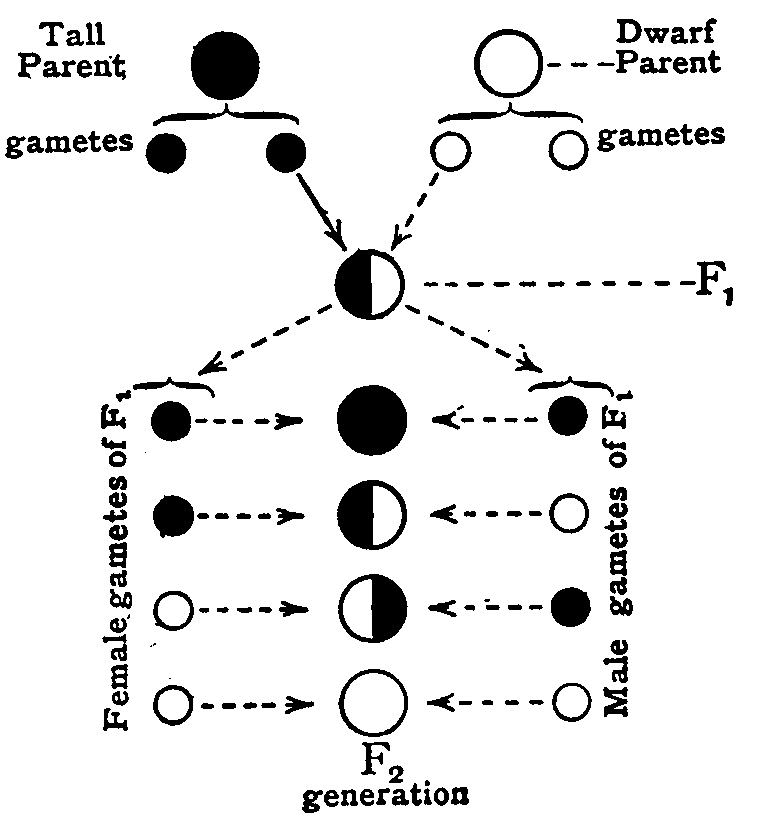
\includegraphics[keepaspectratio, width  =\textwidth]{img/Pgen_to_F2}
			\end{column}
		\end{columns}

			\blfootnote{Figure from Punnett 1911}
			
	\end{frame}
	
	
	\begin{frame}
		\frametitle{Outline for Today}
		\setbeamertemplate{itemize items}[circle]
		\Large{
			\begin{itemize} 
				\item Chromosomes and Their Structure
				\item Linkage \& Genetic Mapping
				\item DNA 
			\end{itemize}
		}
		
		\note{
			Learning Outcomes
			\emph{		\begin{itemize} 
					\item Basic definitions in genetics
					\item Principles and terms in classical genetics
					\item Molecular mechanisms of classical genetics
					\item Chromosome crossover and its significance
				\end{itemize}
			}
		}
	\end{frame}
	
	
\begin{frame}
	\frametitle{Chromosomes}
\Large \centering	Chromsosomes are the ``particles of inheritence", but what are they?

	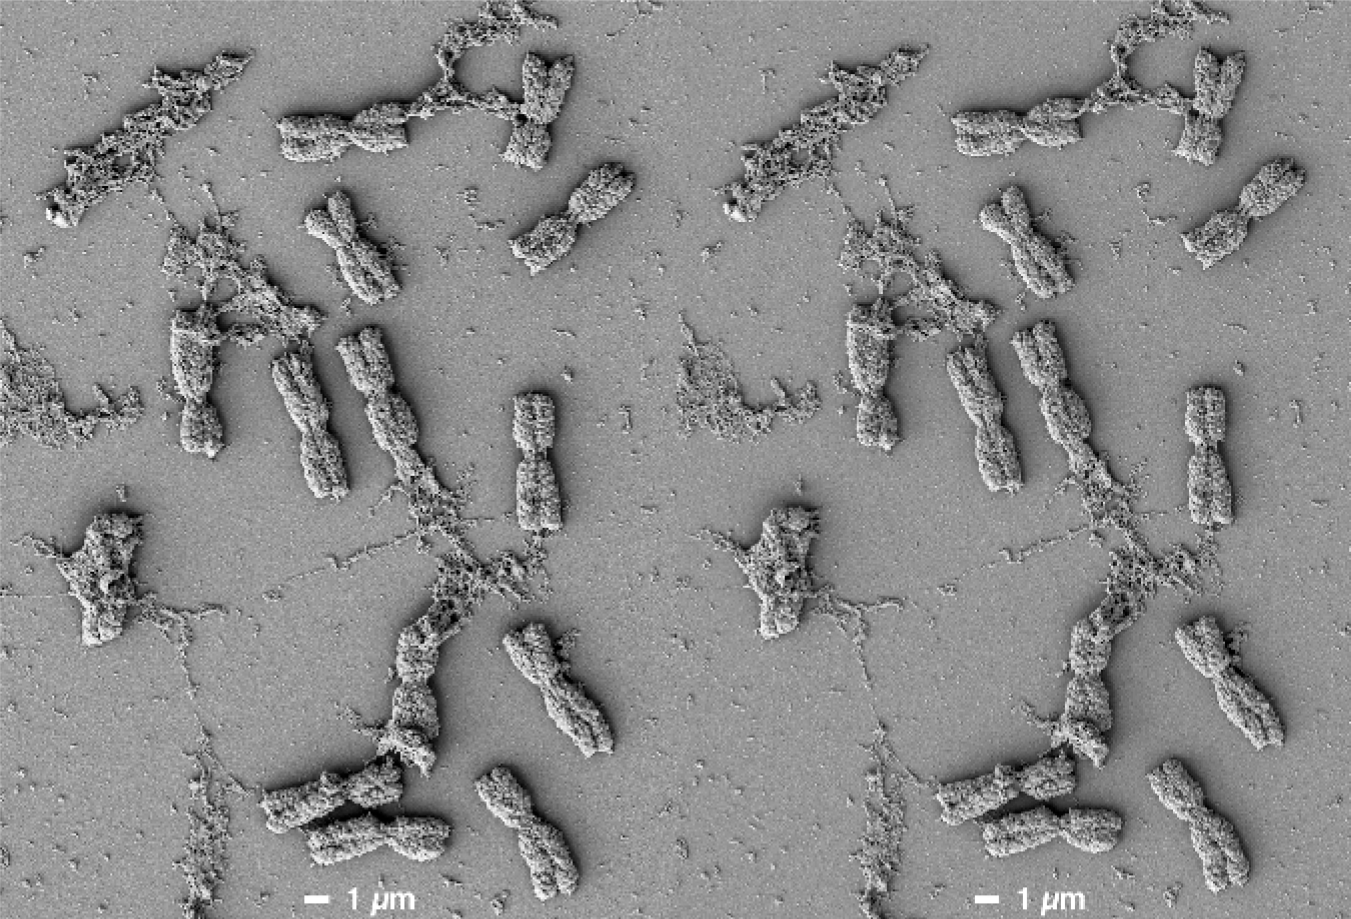
\includegraphics[keepaspectratio, width  =0.8\textwidth]{img/barleyChroms}\blfootnote{SEM of barley chromosomes in metaphase: Schroeder-Reiter and Wanne 2013 \textit{SEM for the Life Sciences}}
	\note{https://www.genome.gov/genetics-glossary/Chromatin}
\end{frame}	
	
\begin{frame}
	\frametitle{Chromosome Structure}
\begin{columns}
	\begin{column}{0.5\textwidth}

\centering	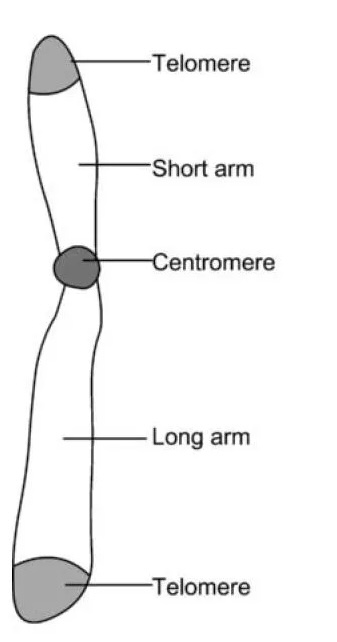
\includegraphics[keepaspectratio, width  =0.8\textwidth]{img/chromosomeDiagram} \pause
	\end{column}
	\begin{column}{0.5\textwidth}
	\centering	Centromeres play a structural in meiosis\\
	\vspace{5pt}	
		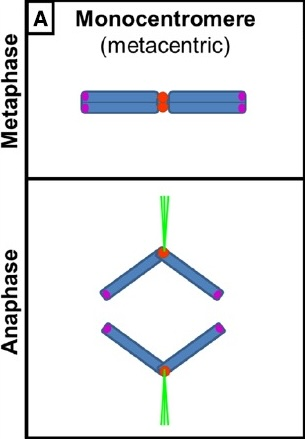
\includegraphics[keepaspectratio, width  =0.75\textwidth]{img/centromeresInAction} \blfootnote{Modified from \textit{Cuacos et al 2015 Front. Plant Sci.} }
		\end{column}
		
\end{columns}

\end{frame}	
	
	
	\begin{frame}
		\frametitle{Chromosome Types}
		\begin{columns}
			\begin{column}{0.5\textwidth}
				
				\centering	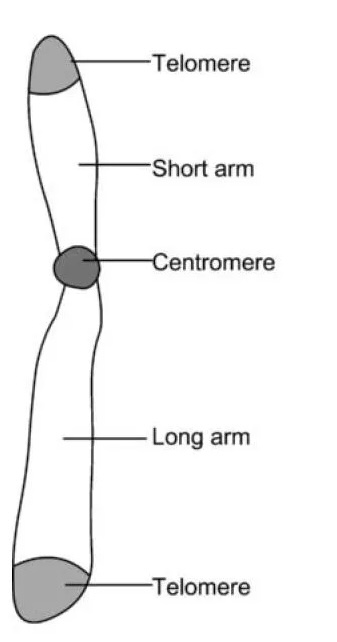
\includegraphics[keepaspectratio, width  =0.8\textwidth]{img/chromosomeDiagram} 
			\end{column}
			\begin{column}{0.5\textwidth}
				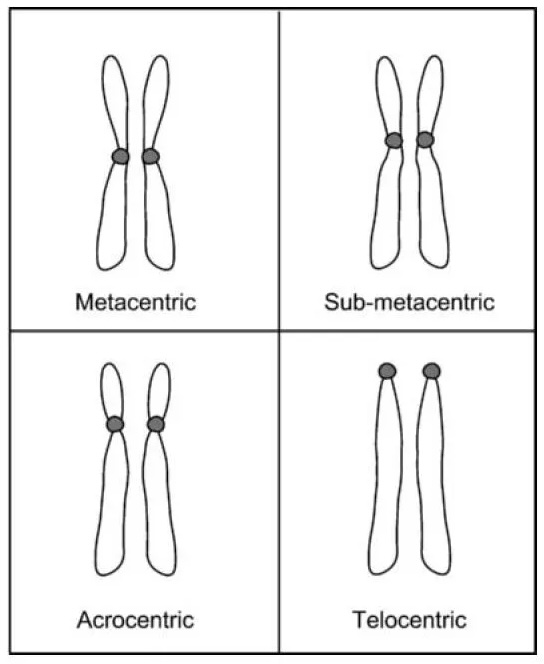
\includegraphics[keepaspectratio, width  =0.8\textwidth]{img/chromosomeTypes} 
			\end{column}
			
		\end{columns}
		
	\end{frame}	
	
\begin{frame}
		\frametitle{Chromosome Numbers}
		\begin{columns}
			\begin{column}{0.5\textwidth}
The number of sets of homologous chromosome organisms possess varies widely!

 \begin{itemize}[leftmargin=100pt]
	\item[\textbf{Humans}] 23 
	\item[\textbf{Maize}] 10 
	\item[\textbf{Banana}] 11
	\item[\textbf{Loblolly pine}] 12
\end{itemize}
\note{The record holder is 227 for the Atlantic Blue Butterfly - though this of course may be beaten}

\textit{There is no known correlation between organisms complexity and chromosome count}
			\end{column}
			\begin{column}{0.5\textwidth}
\pause
	Douglas-fir has 13 chromosomes, but recently underwent a chromsome fission\\
	\centering
		\includegraphics[keepaspectratio, width  =0.5\textwidth]{img/DouglasFirKaryotype}\blfootnote{Idiogram from Doerksen and Ching 1972 \textit{Forest Science}}
	
			\end{column}
		\end{columns}
		
		\end{frame}
	
	
	
	
	
\begin{frame}
	\frametitle{Chromosomes - Ploidy}
	
	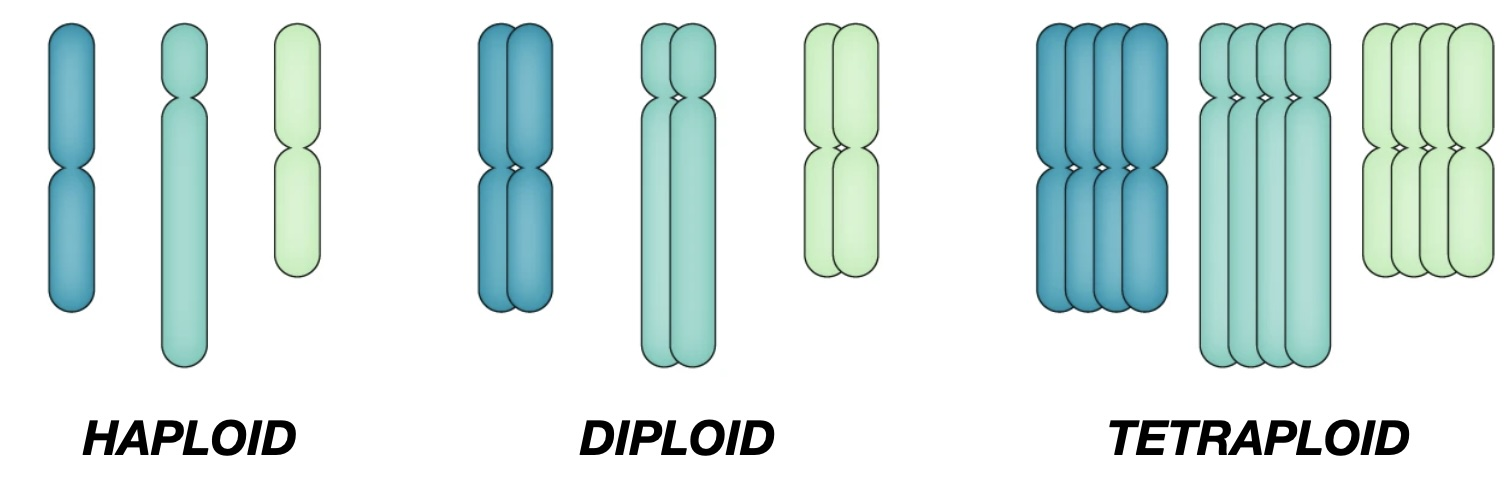
\includegraphics[keepaspectratio, width  =\textwidth]{img/ploidy}
	Ploidy refers to thenumber of homologous chromosome copies an organism possesses\\
	Differences in ploidy are extremely common in plants.
\pause	
\bigskip
\begin{columns}
	\begin{column}{0.2\textwidth}
		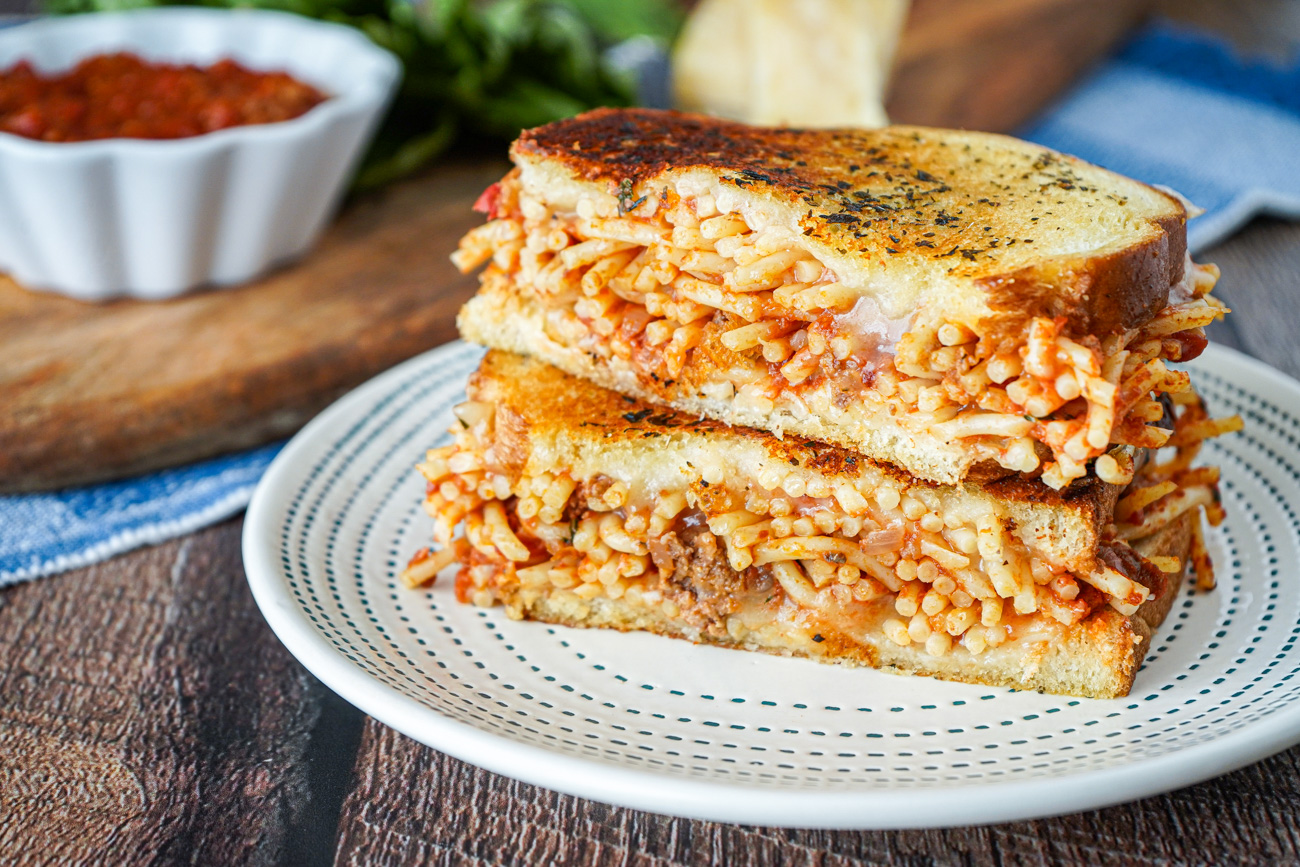
\includegraphics[keepaspectratio, width  =\textwidth]{img/spaghettiSandwich}
\end{column}	
\begin{column}{0.8\textwidth}
	Pasta wheat is tetraploid (4n) and bread wheat is hexapoid (6n)!
	\end{column}
\end{columns}
\end{frame}
	
\begin{frame}
	\frametitle{Sex Chromosomes}
	\begin{columns}
		\begin{column}{0.7\textwidth}
				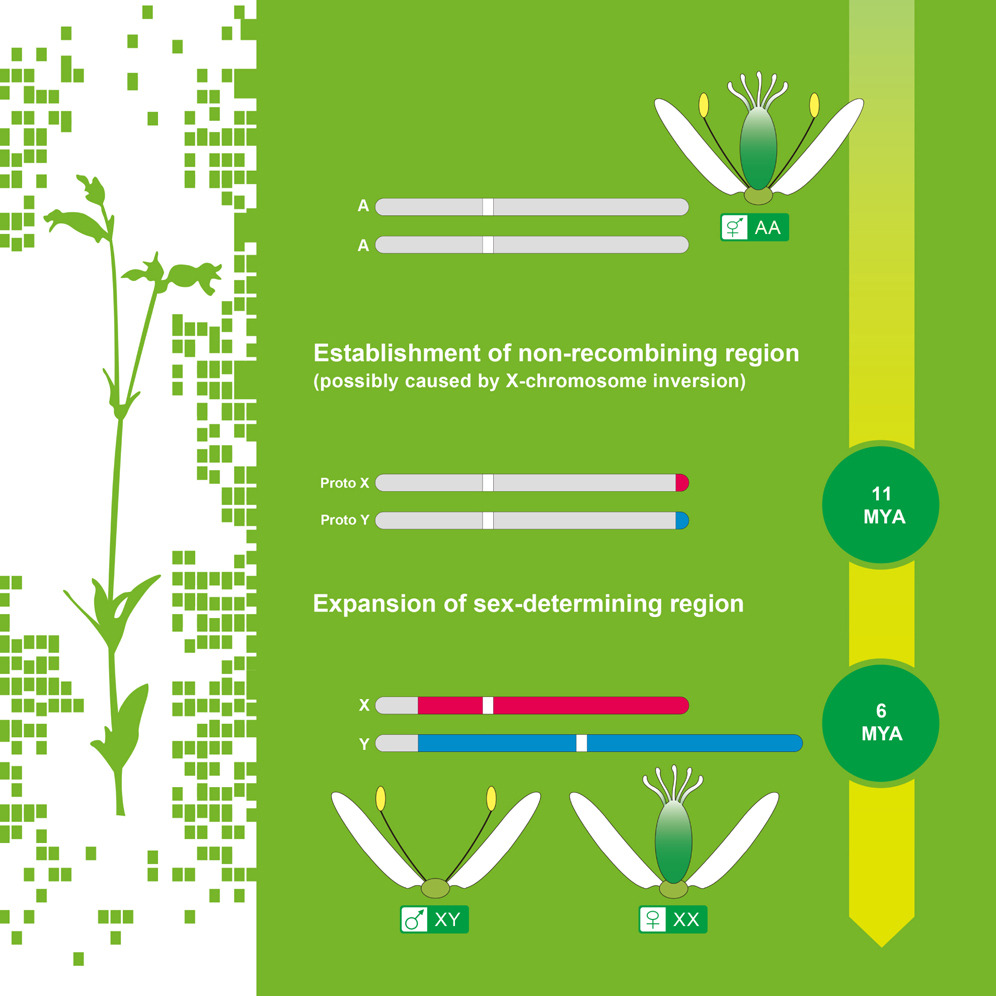
\includegraphics[keepaspectratio, width  =\textwidth]{img/sileneSexChroms}
		\end{column}
		\begin{column}{0.3\textwidth}
				\small In many organisms, specific chromosomes or chromosomal regions are linked to the expression of sex-specific traits.\\
				\vspace{20pt}
				\small  \textit{Silene latifolia}, for example, has an XY sex-chromosome system
				
				
			\end{column}
	\end{columns}
\blfootnote{Yue et al 2023 -\textit{Current Biology}}
\end{frame}
	
	\begin{frame}
		\frametitle{Mendel's Laws}
		
		Refresher... \\
		
		
		\textbf{The law of segregation: } each individual possesses a pair of particles for any particular trait and each parent passes one of these randomly to its offspring \pause
		
		\vspace{10pt}
		
		\textbf{The law of dominance: } for some traits, the presence of one kind of particle masks the presence of another. Mendel referred to the \textbf{dominant} particle as masking the effects of the \textbf{recessive} particle \pause
		
		\vspace{10pt}
		
		\textbf{The law of independant assortment:} when two individuals differ in more than two pairs of traits (e.g. smooth v. wrinkly and green v. yellow), the inheritance of one pair of traits is independent of another 
		
	\end{frame}
	
	
	\begin{frame}
		
		\frametitle{Dihybrid Cross}
		
		In the last lecture, we restricted ourselves to looking at the expected ratios of genotypes for a single trait in a given cross, but there's no reason we need to do that\\
		\bigskip
		Let's now follow the inheritence of two traits instead and stick with smooth v. wrinkly and yellow v. green\\ \pause
		
\center{					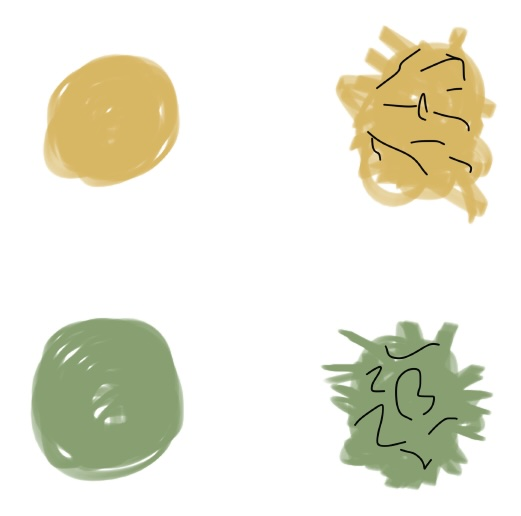
\includegraphics[keepaspectratio, width  =0.45\textwidth]{img/dihybridPeas} }\\
	 	

	 	
%		\begin{tabular}{c|c|c|c|}
%			\multicolumn{2}{c|}{} & \multicolumn{2}{c|}{\textbf{GG}} \\
%			\multicolumn{2}{c|}{} & \textbf{G} & \textbf{G} \\
%			\hline 
%			\multirow{2}{*}{\textbf{YG}}	& \textbf{G}& GG& GG \\		
%			\cline{2-4} 
%			&	\textbf{Y} & YG & GY \\
%			\hline
%		\end{tabular}
		
		
	\end{frame}
	
	

	\begin{frame}
		
		\frametitle{Dihybrid cross}
			
	Let's cross ``true breeding" peas that were smooth and yellow with peas that are wrinkly and green
	
\begin{center}
	 	Parental Generation:$
	 	\begin{array}{l}
	 		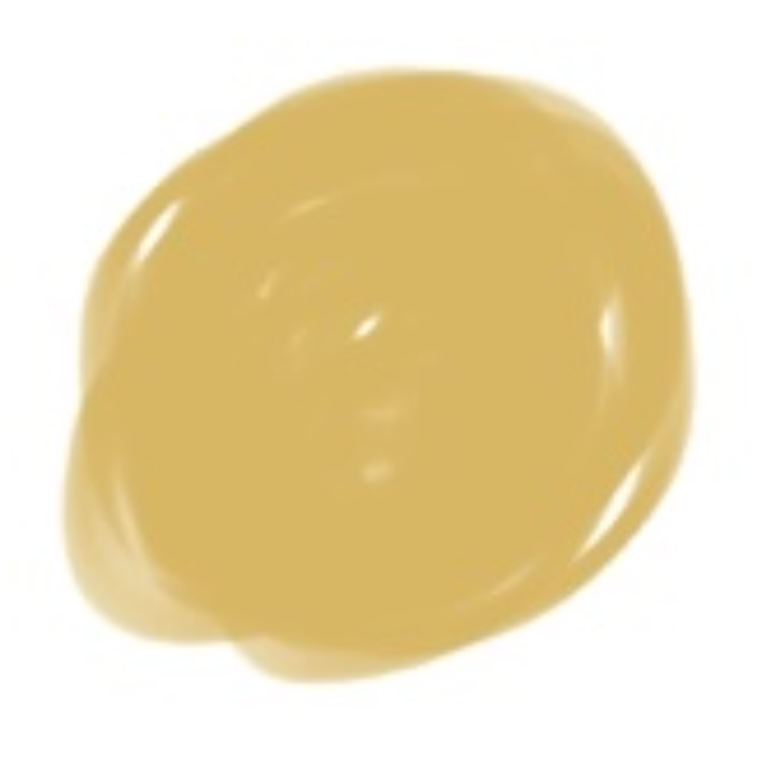
\includegraphics[width=0.1\textwidth]{img/yellowSmooth}
	 	\end{array}
	 	$
	 	$x$
	 	$
	 	\begin{array}{l}
	 		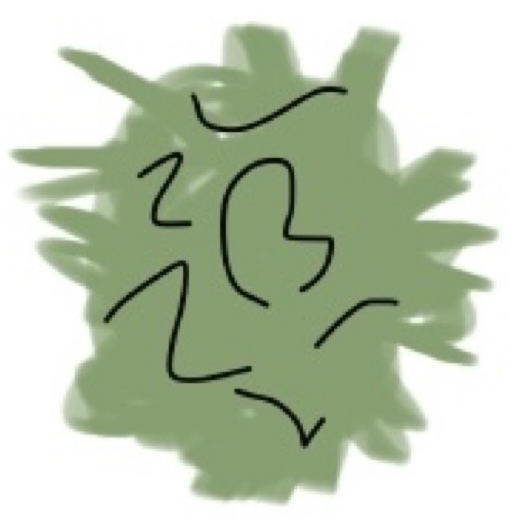
\includegraphics[width=0.1\textwidth]{img/wrinklyGreen}
	 	\end{array}
	 	$\\
	 	
	 \hspace{14.2mm}	Genotypes: YYWW $x$ yyww \\ \pause
	 \vspace{5pt}
	 	\hspace{47mm} $\downarrow$
	
	\hspace{23pt} F1 Generation:$
\begin{array}{l}
	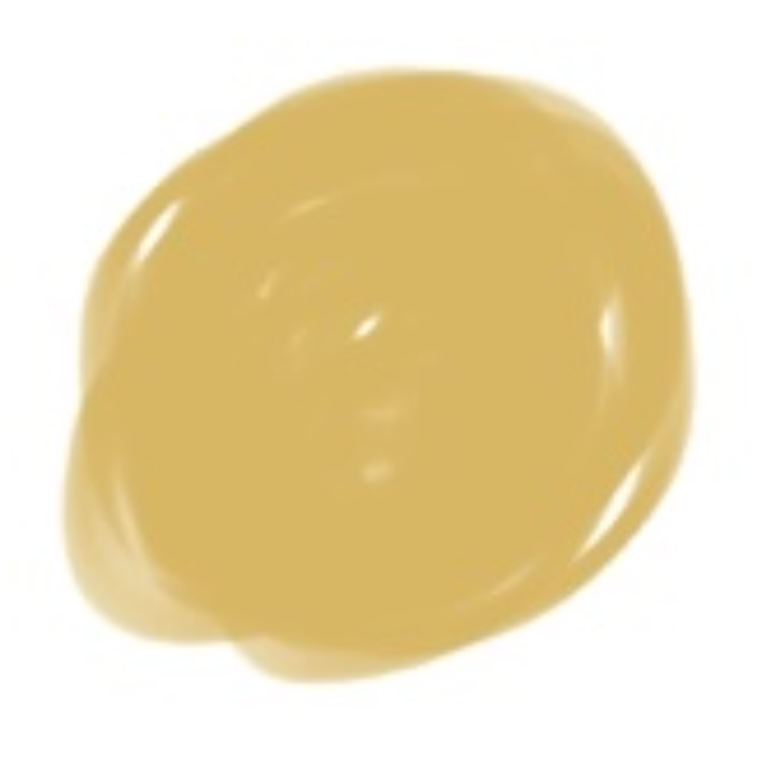
\includegraphics[width=0.1\textwidth]{img/yellowSmooth}
\end{array}
$
$x$
$
\begin{array}{l}
	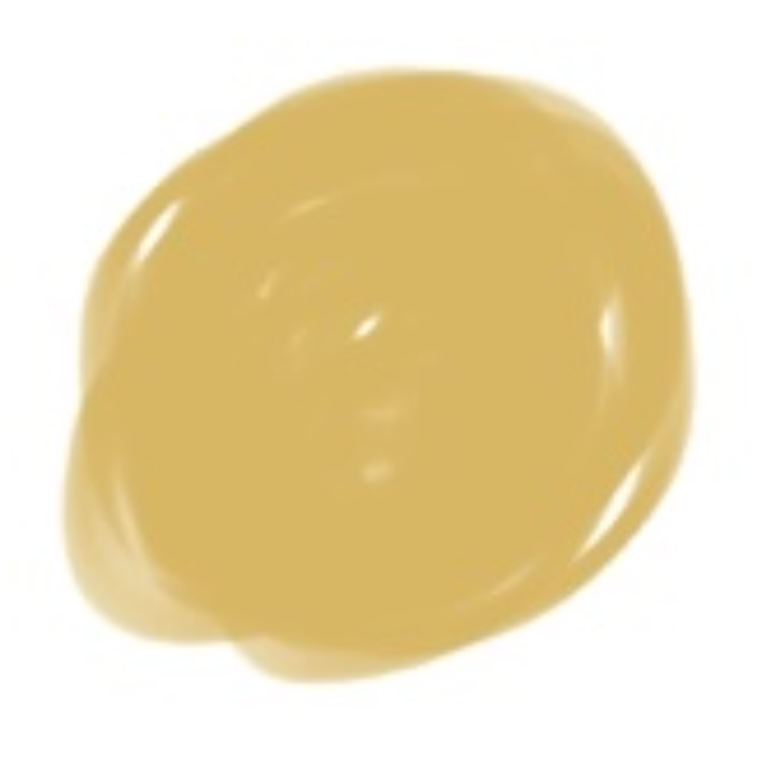
\includegraphics[width=0.1\textwidth]{img/yellowSmooth}
\end{array}
$\\

\hspace{14.2mm}	Genotypes: \textcolor[HTML]{E1BE6A}{\textbf{YyWw}} $x$ \textcolor[HTML]{40B0A6}{\textbf{YyWw}} \\
\vspace{5pt}
\end{center}
		\end{frame}
		%E1BE6A
		%40B0A6
\begin{frame}
	\frametitle{Dihybrid Cross}
If we filled out the Punnett square for this cross, what would the expected ratio of phenotypic combinations be?\\
 
 \bigskip

\begin{tabular}{c|c|c|c|c|c|}
	\multicolumn{2}{c|}{} & \multicolumn{4}{c}{	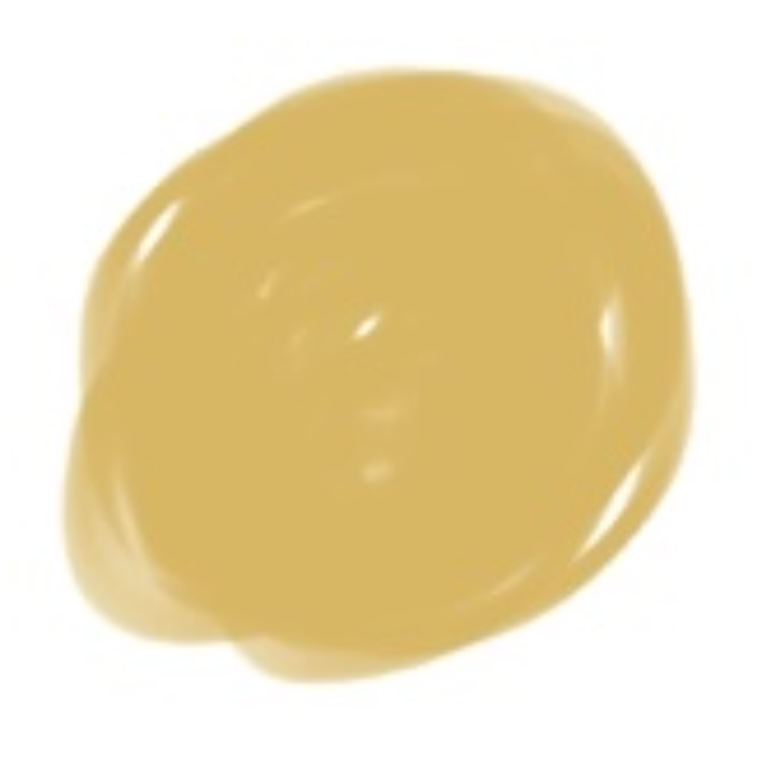
\includegraphics[width=0.1\linewidth]{img/yellowSmooth} \textcolor[HTML]{E1BE6A}{\textbf{YyWw}}} \\
		\cline{3-6} 
	\multicolumn{2}{c|}{} & \textcolor[HTML]{E1BE6A}{\textbf{YW}} &  \textcolor[HTML]{E1BE6A}{\textbf{Yw}}&  \textcolor[HTML]{E1BE6A}{\textbf{yW}} &  \textcolor[HTML]{E1BE6A}{\textbf{yw}}\\
	\hline 
	\multirow{2}{*}{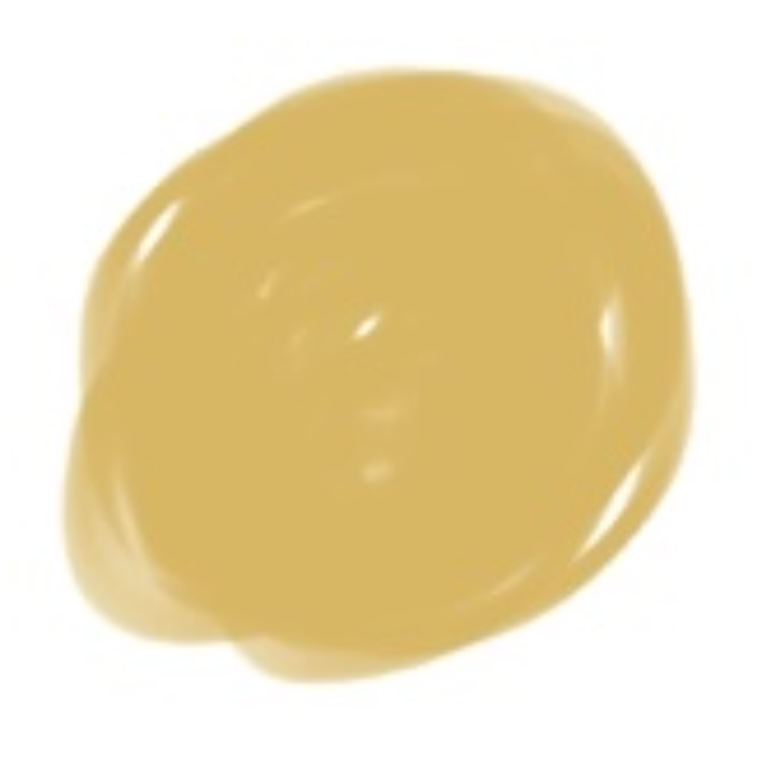
\includegraphics[width=0.1\linewidth]{img/yellowSmooth} }	& \textcolor[HTML]{40B0A6}{\textbf{YW}}& &  & &\\		
	\cline{2-6} 
	&	\textcolor[HTML]{40B0A6}{\textbf{Yw}} & &  & &\\
		\cline{2-6} 
		\multirow{2}{*}{\textcolor[HTML]{40B0A6}{\textbf{YyWw}}}&	\textcolor[HTML]{40B0A6}{\textbf{yW}} & &  & &\\
		\cline{2-6} 
	&	\textbf{\textcolor[HTML]{40B0A6}{\textbf{yw}}} & &  & & \\
		\cline{1-6} 
\end{tabular}

	
\end{frame}
	
	\begin{frame}
		\frametitle{Dihybrid Cross}
	
		\begin{tabular}{c|c|c|c|c|c|}
			\multicolumn{2}{c|}{} & \multicolumn{4}{c}{	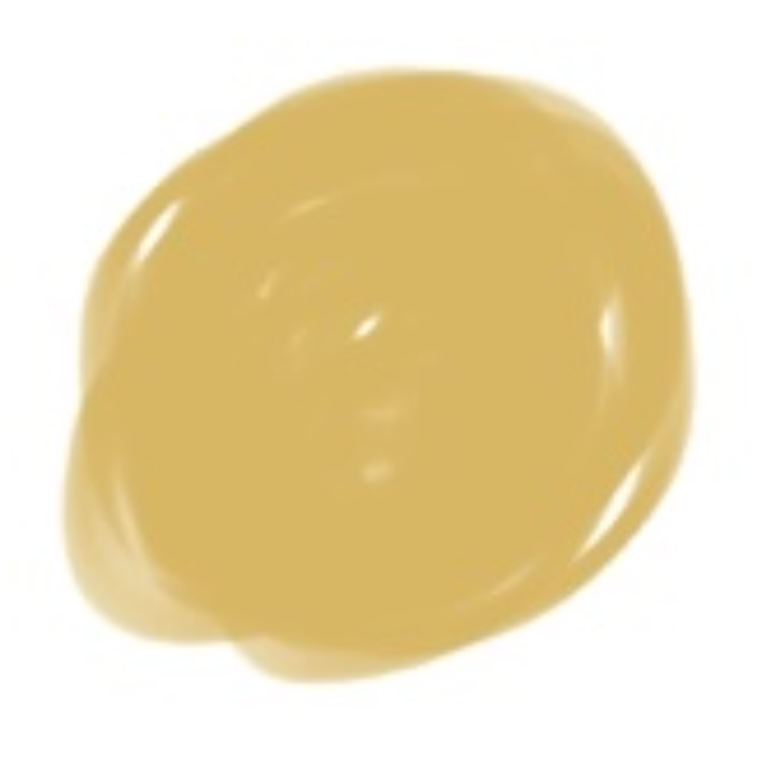
\includegraphics[width=0.1\linewidth]{img/yellowSmooth} \textcolor[HTML]{E1BE6A}{\textbf{YyWw}}} \\
			\cline{3-6} 
			\multicolumn{2}{c|}{} & \textcolor[HTML]{E1BE6A}{\textbf{YW}} &  \textcolor[HTML]{E1BE6A}{\textbf{Yw}}&  \textcolor[HTML]{E1BE6A}{\textbf{yW}} &  \textcolor[HTML]{E1BE6A}{\textbf{yw}}\\
			\hline 
			%Line 1
			\multirow{2}{*}{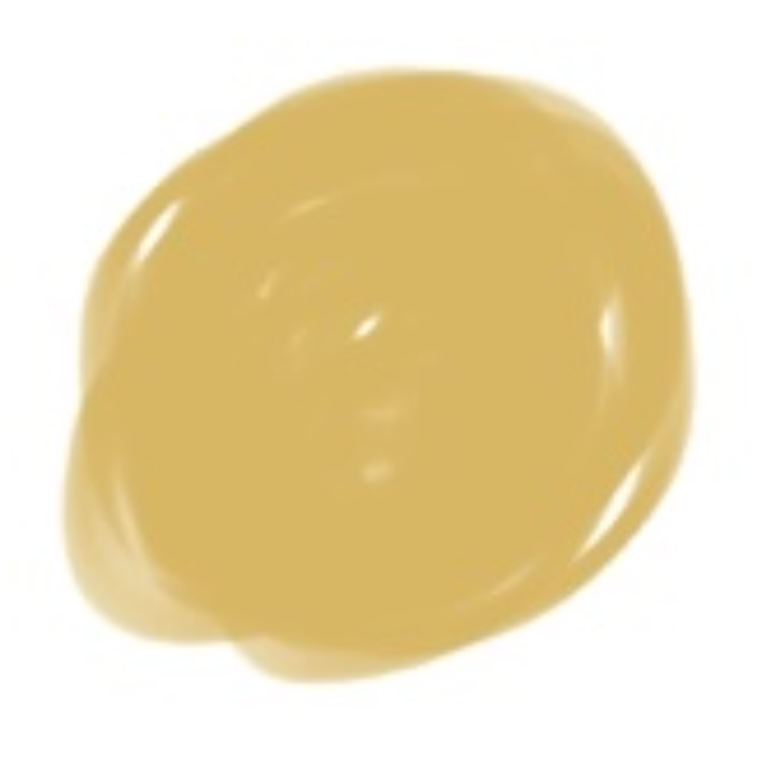
\includegraphics[width=0.1\linewidth]{img/yellowSmooth} }	& \textcolor[HTML]{40B0A6}{\textbf{YW}}&
			\textcolor[HTML]{E1BE6A}{\textbf{Y}}\textcolor[HTML]{40B0A6}{\textbf{Y}}\textcolor[HTML]{E1BE6A}{\textbf{W}}\textcolor[HTML]{40B0A6}{\textbf{W}} &  
			\textcolor[HTML]{E1BE6A}{\textbf{Y}}\textcolor[HTML]{40B0A6}{\textbf{Y}}\textcolor[HTML]{E1BE6A}{\textbf{w}}\textcolor[HTML]{40B0A6}{\textbf{W}} 
			& \textcolor[HTML]{E1BE6A}{\textbf{y}}\textcolor[HTML]{40B0A6}{\textbf{Y}}\textcolor[HTML]{E1BE6A}{\textbf{W}}\textcolor[HTML]{40B0A6}{\textbf{W}} 
			&\textcolor[HTML]{E1BE6A}{\textbf{y}}\textcolor[HTML]{40B0A6}{\textbf{Y}}\textcolor[HTML]{E1BE6A}{\textbf{w}}\textcolor[HTML]{40B0A6}{\textbf{W}} \\		
			\cline{2-6} 
			
			% Line 2
			&	\textcolor[HTML]{40B0A6}{\textbf{Yw}} & 
			\textcolor[HTML]{E1BE6A}{\textbf{Y}}\textcolor[HTML]{40B0A6}{\textbf{Y}}\textcolor[HTML]{E1BE6A}{\textbf{W}}\textcolor[HTML]{40B0A6}{\textbf{w}} &  
			\textcolor[HTML]{E1BE6A}{\textbf{Y}}\textcolor[HTML]{40B0A6}{\textbf{Y}}\textcolor[HTML]{E1BE6A}{\textbf{w}}\textcolor[HTML]{40B0A6}{\textbf{w}} 
			& \textcolor[HTML]{E1BE6A}{\textbf{y}}\textcolor[HTML]{40B0A6}{\textbf{Y}}\textcolor[HTML]{E1BE6A}{\textbf{W}}\textcolor[HTML]{40B0A6}{\textbf{w}} 
			&\textcolor[HTML]{E1BE6A}{\textbf{y}}\textcolor[HTML]{40B0A6}{\textbf{Y}}\textcolor[HTML]{E1BE6A}{\textbf{w}}\textcolor[HTML]{40B0A6}{\textbf{w}}\\
			\cline{2-6} 
			%Line 3
			\multirow{2}{*}{\textcolor[HTML]{40B0A6}{\textbf{YyWw}}}&
			
			\textcolor[HTML]{40B0A6}{\textbf{yW}} &
			\textcolor[HTML]{E1BE6A}{\textbf{Y}}\textcolor[HTML]{40B0A6}{\textbf{y}}\textcolor[HTML]{E1BE6A}{\textbf{W}}\textcolor[HTML]{40B0A6}{\textbf{W}} &  
			\textcolor[HTML]{E1BE6A}{\textbf{Y}}\textcolor[HTML]{40B0A6}{\textbf{y}}\textcolor[HTML]{E1BE6A}{\textbf{w}}\textcolor[HTML]{40B0A6}{\textbf{W}} 
			& \textcolor[HTML]{E1BE6A}{\textbf{y}}\textcolor[HTML]{40B0A6}{\textbf{y}}\textcolor[HTML]{E1BE6A}{\textbf{W}}\textcolor[HTML]{40B0A6}{\textbf{W}} 
			&\textcolor[HTML]{E1BE6A}{\textbf{y}}\textcolor[HTML]{40B0A6}{\textbf{y}}\textcolor[HTML]{E1BE6A}{\textbf{w}}\textcolor[HTML]{40B0A6}{\textbf{W}}\\
			\cline{2-6} 
			&	\textbf{\textcolor[HTML]{40B0A6}{\textbf{yw}}} & 
			\textcolor[HTML]{E1BE6A}{\textbf{Y}}\textcolor[HTML]{40B0A6}{\textbf{y}}\textcolor[HTML]{E1BE6A}{\textbf{W}}\textcolor[HTML]{40B0A6}{\textbf{w}} &  
			\textcolor[HTML]{E1BE6A}{\textbf{Y}}\textcolor[HTML]{40B0A6}{\textbf{y}}\textcolor[HTML]{E1BE6A}{\textbf{w}}\textcolor[HTML]{40B0A6}{\textbf{w}} 
			& \textcolor[HTML]{E1BE6A}{\textbf{y}}\textcolor[HTML]{40B0A6}{\textbf{y}}\textcolor[HTML]{E1BE6A}{\textbf{W}}\textcolor[HTML]{40B0A6}{\textbf{w}} 
			&\textcolor[HTML]{E1BE6A}{\textbf{y}}\textcolor[HTML]{40B0A6}{\textbf{y}}\textcolor[HTML]{E1BE6A}{\textbf{w}}\textcolor[HTML]{40B0A6}{\textbf{w}} \\
			\cline{1-6} 
		\end{tabular}\\
		\bigskip
		In what proportions would we expect to see the different phenotypic combinations?\\
		\centering
		$
			 	\begin{array}{l}
			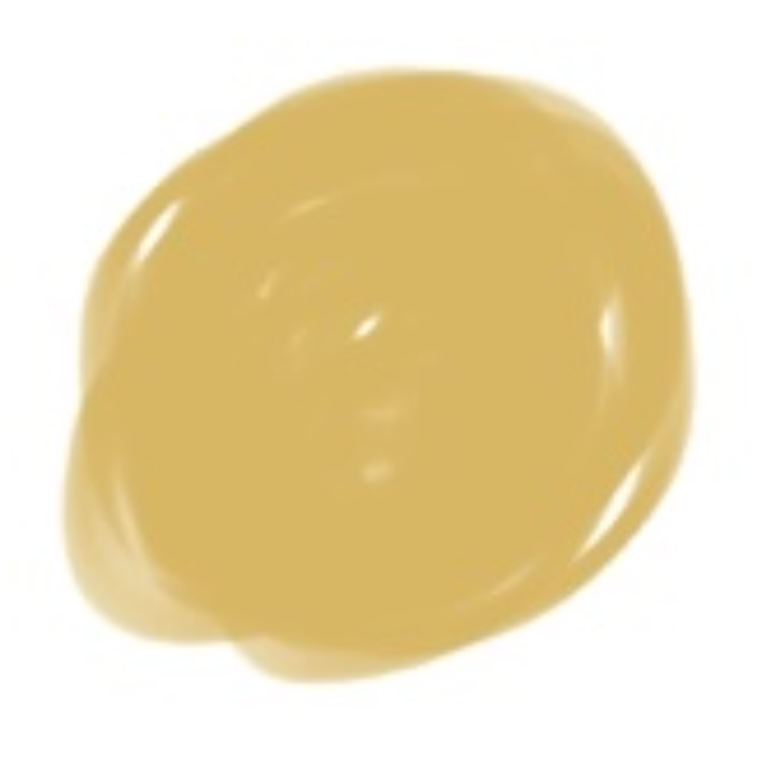
\includegraphics[width=0.1\textwidth]{img/yellowSmooth}
		\end{array}
		$
		$:$
		$
		\begin{array}{l}
			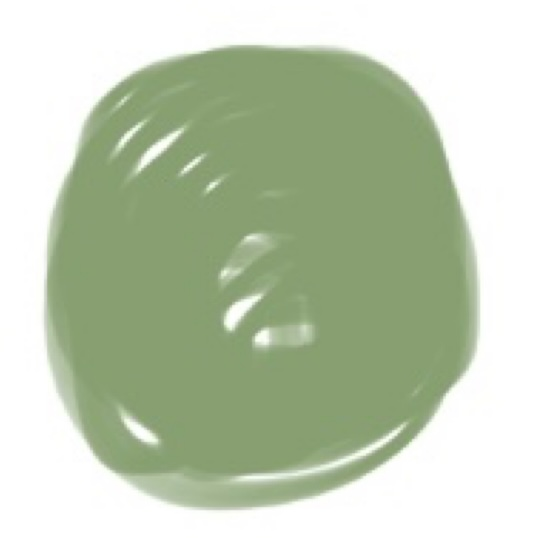
\includegraphics[width=0.1\textwidth]{img/smoothGreen}
		\end{array}
		$
				$:$
		$
		\begin{array}{l}
			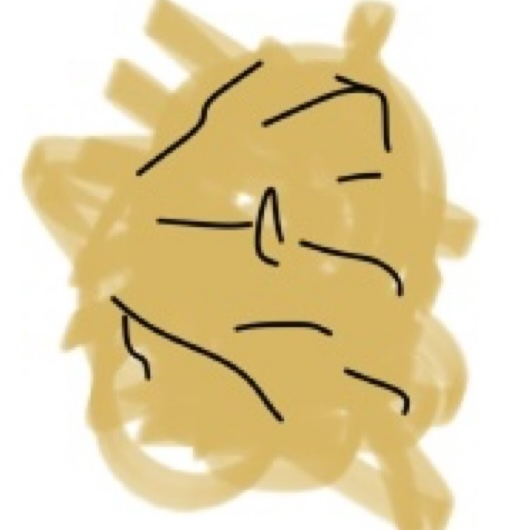
\includegraphics[width=0.1\textwidth]{img/wrinklyYellow}
		\end{array}
		$
				$:$
		$
		\begin{array}{l}
			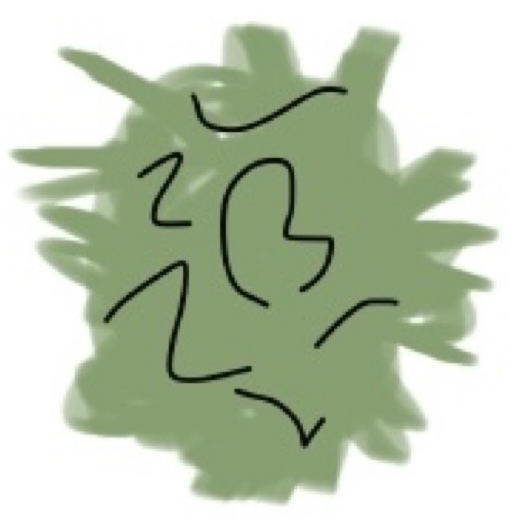
\includegraphics[width=0.1\textwidth]{img/wrinklyGreen}
		\end{array}
		$\\
		

		

	\end{frame}
	
	\begin{frame}
		\frametitle{Dihybrid Cross}
		
	According to the \textbf{Law of Independent Assortment}, we would expect: \\
		$9 x
	\begin{array}{l}
		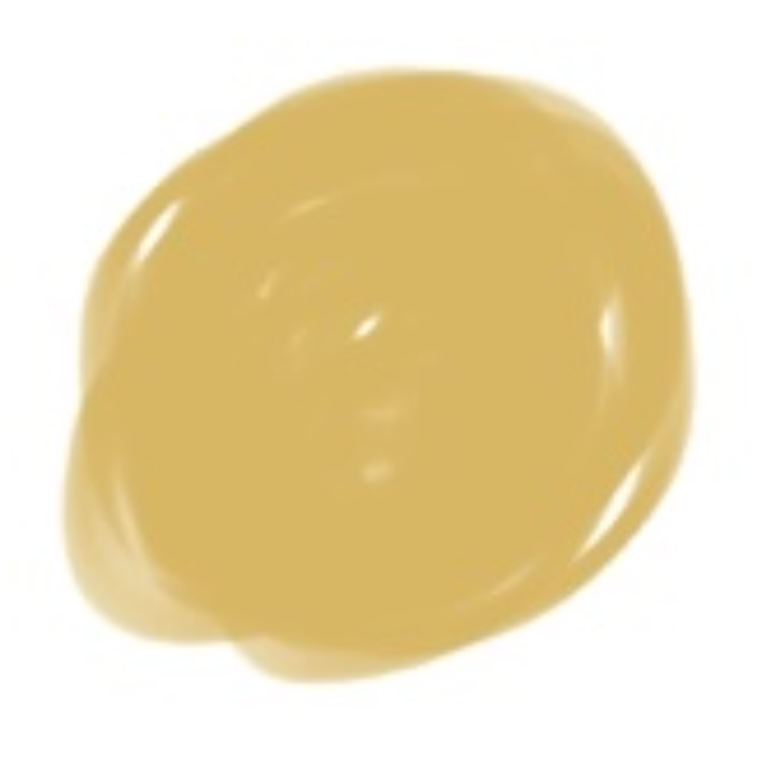
\includegraphics[width=0.1\textwidth]{img/yellowSmooth}
	\end{array}
	$
	$:$
	$
	3 x
	\begin{array}{l}
		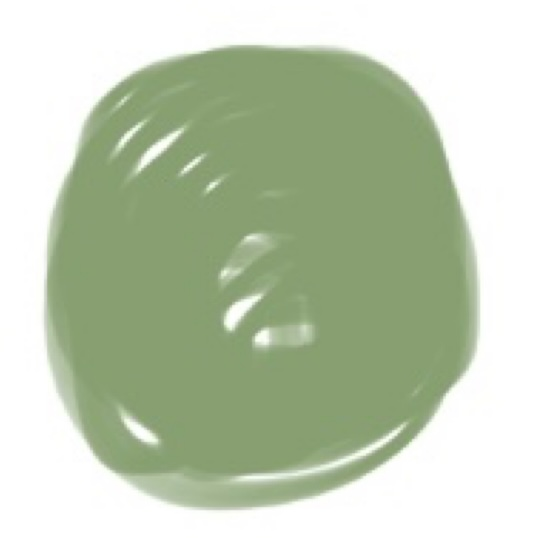
\includegraphics[width=0.1\textwidth]{img/smoothGreen}
	\end{array}
	$
	$:$
	$
	3 x
	\begin{array}{l}
		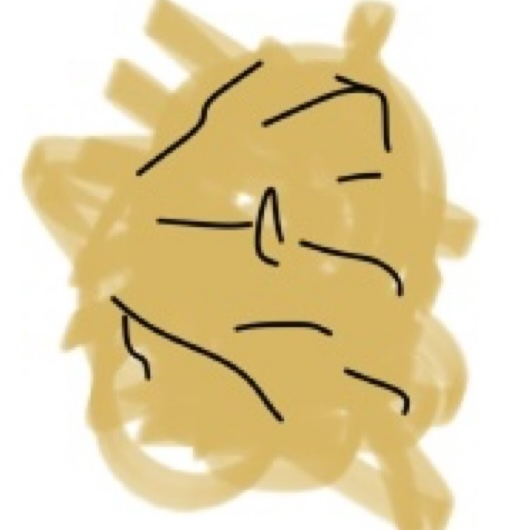
\includegraphics[width=0.1\textwidth]{img/wrinklyYellow}
	\end{array}
	$
	$:$
	$
	1 x
	\begin{array}{l}
		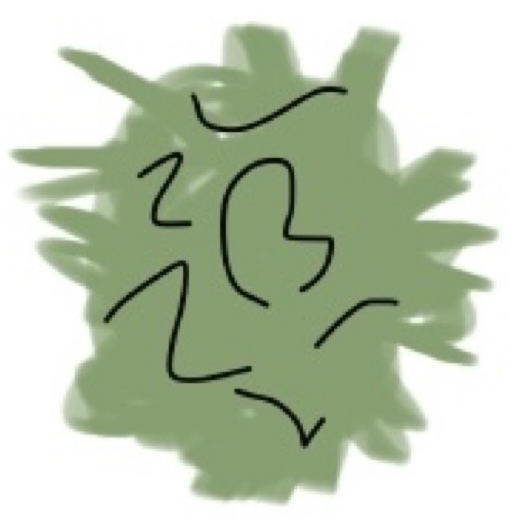
\includegraphics[width=0.1\textwidth]{img/wrinklyGreen}
	\end{array}
	$\\
	

	
	
	\end{frame}
	
	
	\begin{frame}
\frametitle{Results of a Dihybrid Cross in Sweetpeas}		

In the early 1900s, Bateson and Saunders conducted a series of experiments using sweet peas (\textit{Lathyrus odoratus} - not garden peas like Mendel) \\
\vspace{5pt}
Rather than seed colour and texture, they were examining flower colour and the shape of pollen grains\\
\vspace{5pt}
They conducted a dihybrid cross and got the following results:\\
\vspace{8pt}
\begin{center}
\begin{columns}

	\begin{column}{0.5\textwidth}
	\begin{tabular}{c|c}
		\textbf{Phenotype} & \textbf{Observed } \\
		\hline
		\textit{Purple, long}& 1528\\
		
		\textit{Purple, round}&106\\
		
		\textit{Red, long}&117\\
		
		\textit{Red, round}&381\\
		\hline
		\textbf{Total} & 2132\\
	\end{tabular}	

\end{column}
	\begin{column}{0.5\textwidth}
			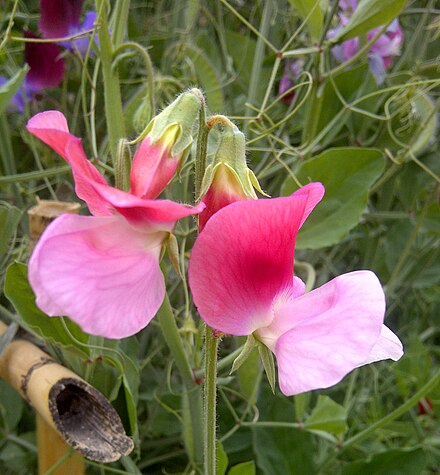
\includegraphics[keepaspectratio, width  =0.75\textwidth]{img/sweetPea} 
	
	\note{source of pic}
\end{column}
\end{columns}
\end{center}


\end{frame}
	
		
		
		\begin{frame}
\frametitle{Results of a Diybrid Cross in Sweetpeas}
With 2132 plants and an expected phenotypic proportions of $9:3:3:1$, we can quantify how strange the deviations from the expectations are\bigskip

\begin{tabular}{c|c|c|>{\onslide<2->}c<{\onslide}}
	\textbf{Phenotype} & \textbf{Expected} & \textbf{Observed } & \textbf{(Obs.-Exp.)\textsuperscript{2}/Exp.}\\
	\hline
	\textit{Purple, long}& 1199 &1528&90.3\\
	
	\textit{Purple, round}&400&106&216.1\\
	
	\textit{Red, long}&400 &117&202.2\\
	
	\textit{Red, round}&133&381&462.4\\
	\hline
	\textit{\textbf{Total}}&2132&2132& $\chi^2 = 969.0$\\
	
	
		\hline
\end{tabular}	

{\onslide<2->}\small{This $\chi^2$ test gives a $p-$value $< 0.0001$}{\onslide}

\blfootnote{Results from: \textit{Bateson, W., Saunders et al. Experimental studies in the physiology of heredity. Reports to the Evolution Committee of the Royal Society 2, 1–55, 80–99 (1905)}}
		\end{frame}
		
		\begin{frame}
			
			\huge \textit{Q: Why would we see deviations from the Law of Independant Assortment?} \pause
			
			\Huge \textbf{A: Linkage!}
			
			
		\end{frame}
		
		
		
	
		
\begin{frame}


	
	\frametitle{Genetic Linkage}
	
	\centering 				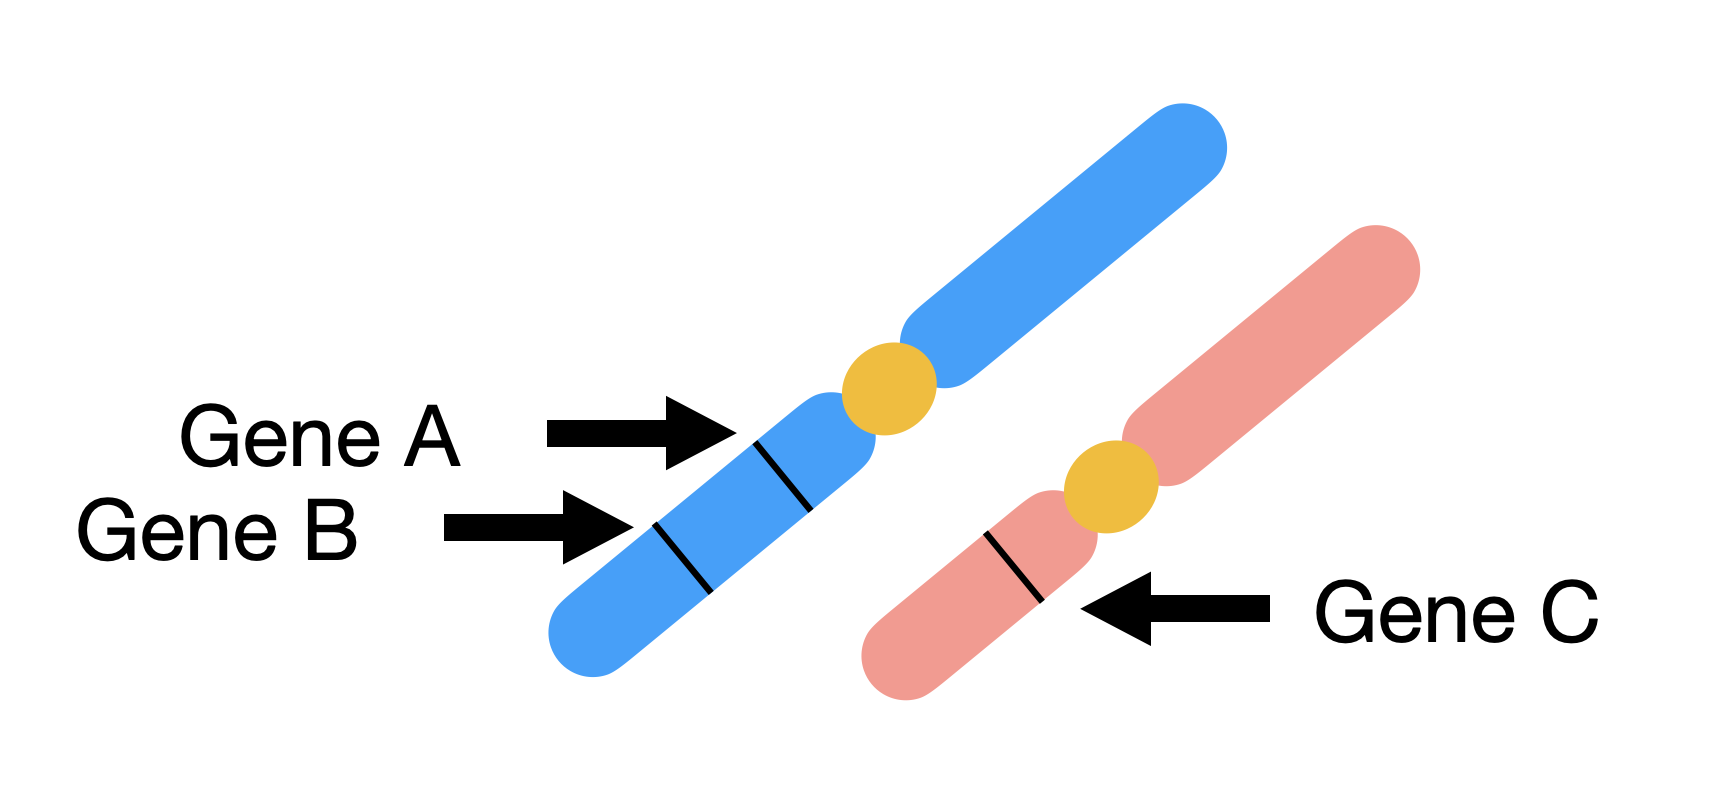
\includegraphics[keepaspectratio, width  =0.7\textwidth]{img/linkageCartoon} \\
	
\small 
\begin{itemize}
		\item[--] The law of the independent assortment was derived based on genes located\textbf{ on different chromosomes}. Alleles of these genes \textbf{segregate independently }during meiosis \pause

		\item[--] Genes located on the same chromosome may be inherited together during meiosis \pause
		
		\item[--] But this is inadequate to explain the emergence of new trait combinations in the sweet peas
		
	\end{itemize}
\blfootnote{Figure from:\textit{ Brown 2002}}
\end{frame}
		
		
		
		
		

\begin{frame}
	\frametitle{Crossing Over}
\begin{columns}
	
	\begin{column}{0.45\textwidth}
\begin{itemize}
\small 
	\item [--]  In the 1910s, Thomas Hunt Morgan developed genetic experiments with the fruit fly 	\textit{Drosophila melanogaster}
		\item [--] Morgan and colleagues observed cases where expected ratios for linked factors broke down (just like with the sweet peas)
			\item [--] They proposed a process of ``\textit{crossing-over}" where alleles may swap onto alternate chromosome pairs
	
\end{itemize}	
		\end{column}
	\begin{column}{0.6\textwidth}
				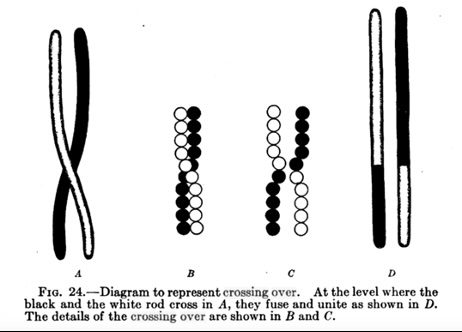
\includegraphics[keepaspectratio, width  =\textwidth]{img/MorganCrossover} 

	\end{column}
\end{columns}
	\blfootnote{Image from \textit{Morgan, T.H., Sturtevant, A.H., and Bridges, C.B. (1915). The Mechanism of Mendelian heredity}.}
\note{Crossing over was first discovered in 1909, but it's effects on inheritence were not validated until the 1930s by Barbara McClintock - and this was not even what McClintock won the Nobel prize for!!!}	
\end{frame}






\begin{frame}
	\frametitle{Linkage in Sweet Peas}		
	
	
	\begin{center}
		\begin{columns}
			
			\begin{column}{0.5\textwidth}
				\centering						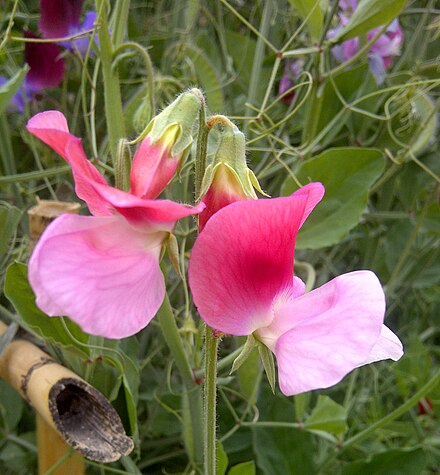
\includegraphics[keepaspectratio, width  =0.5\textwidth]{img/sweetPea} \\
				
				\vspace{20pt}
				\begin{tabular}{c|c}
					\textbf{Phenotype} & \textbf{Observed } \\
					\hline
					\textit{Purple, long}& 1528\\
					
					\textit{Purple, round}&106\\
					
					\textit{Red, long}&117\\
					
					\textit{Red, round}&381\\
					\hline
					\textbf{Total} & 2132\\
				\end{tabular}	
				
			\end{column}
			\begin{column}{0.5\textwidth}
								\centering \small	Which of the following do you think is the closest approximation of the arrangement of genes in the sweetpea?\\
								\vspace{10pt}
									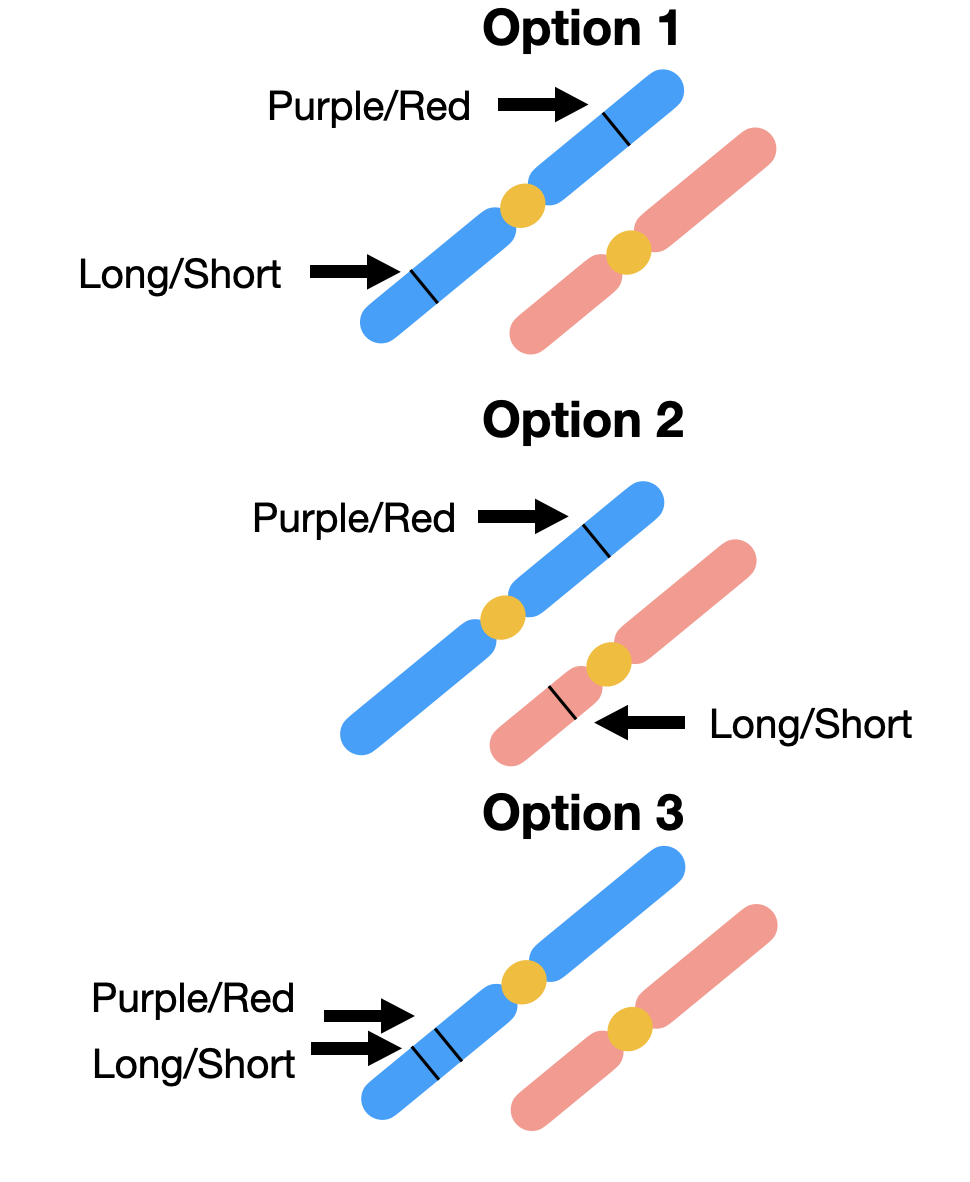
\includegraphics[keepaspectratio, width  =0.9\textwidth]{img/linkageHandsUp} \\
				
				
			\end{column}
		\end{columns}
	\end{center}
	
	
\end{frame}





\begin{frame}
	\frametitle{Crossing Over}
	
	\centering			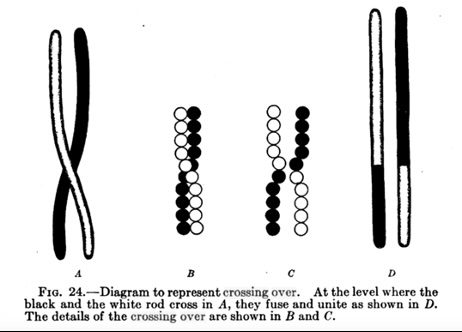
\includegraphics[keepaspectratio, width  =0.8\textwidth]{img/MorganCrossover} \\

	
	\blfootnote{Image from \textit{Morgan, T.H., Sturtevant, A.H., and Bridges, C.B. (1915). The Mechanism of Mendelian heredity}.}
	
	
\end{frame}		
		


\begin{frame}
	\frametitle{Measuring Genetic Distance}
	\begin{columns}
		\begin{column}{0.4\textwidth}
				
\small If we assume that the purple/red and long/round genes are on the same chromosome, we can calculate the genetic distance between them

			\vspace{15pt}
			\begin{tabular}{c|c}
				\textbf{Phenotype} & \textbf{Observed } \\
				\hline
				\textit{Purple, long}& 1528\\
				
				\textit{Purple, round}&106\\
				
				\textit{Red, long}&117\\
				
				\textit{Red, round}&381\\
				\hline
				\textbf{Total} & 2132\\
			\end{tabular}	
			
			
			\end{column}
			\begin{column}{0.7\textwidth}

\small			Number of recombinant genotypes = \pause$106+117$

\small Recombination fraction = $0.105$ \\

\vspace{10pt}

\small We usually express these recombination units as:\\

 $100 \times Recombination Fraction = 10.5cM$
 \vspace{30pt}
 
Where $cM$ stands for centimorgans: the expected number of recombination events observed in 100 meioses

\pause
\vspace{30pt}

What is the maximum genetic distance possible between two markers?


			\end{column}
		\end{columns}
		
	\end{frame}
	

%\small				We express genetic distances\footnote{some refer to genetic dissimilarity among individuals as the \textit{genetic distance}} in terms of the recombination fraction identified between them

%The recombination fraction between two genes is expressed in Morgans (M) - 1M refers to a probability of 				This fraction is expressed in Morgans (M), where 1 M corresponds to the length of DNA on which one recombination is expected on average (roughly equivalent to 100 million bp), but is usually written as centiMorgans (cM), where 1 cM is the genetic distance corresponding to a recombination fraction of 0.01



\begin{frame}
	\frametitle{Genetic Mapping}
	\begin{columns}
		\begin{column}{0.4\textwidth}
			\centering	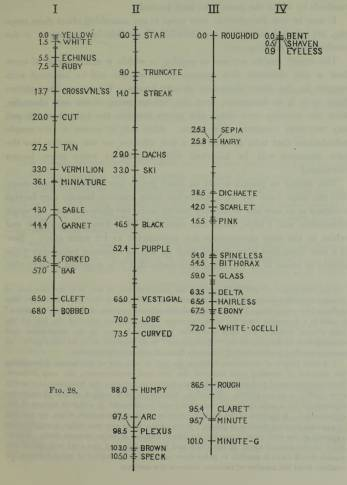
\includegraphics[keepaspectratio, width  =\textwidth]{img/MorganMap} 
		\end{column}
		\begin{column}{0.6\textwidth}
			
			\begin{itemize}			
				\item[--] The frequency of ``crossed-over" trait combinations gave Morgan and colleagues the ability to identify the order of genes on the \textit{D. melanogaster} chromosomes 
				\item[--] More amazingly, they had the insight that the relative frequency of cross-overs could be used to quantify the distance between genes along the chromosomes
				
			\end{itemize}
			
		\end{column}
	\end{columns}
	\blfootnote{Morgan 1922}
	\note{Morgan was awarded the Nobel prize for the discoveries his group made!}
\end{frame}

\begin{frame}
	\frametitle{Douglas-fir Genetic Map}
These principles are the basis of \textbf{genetic mapping}, a technique that is still widely used today\\
	
				\centering	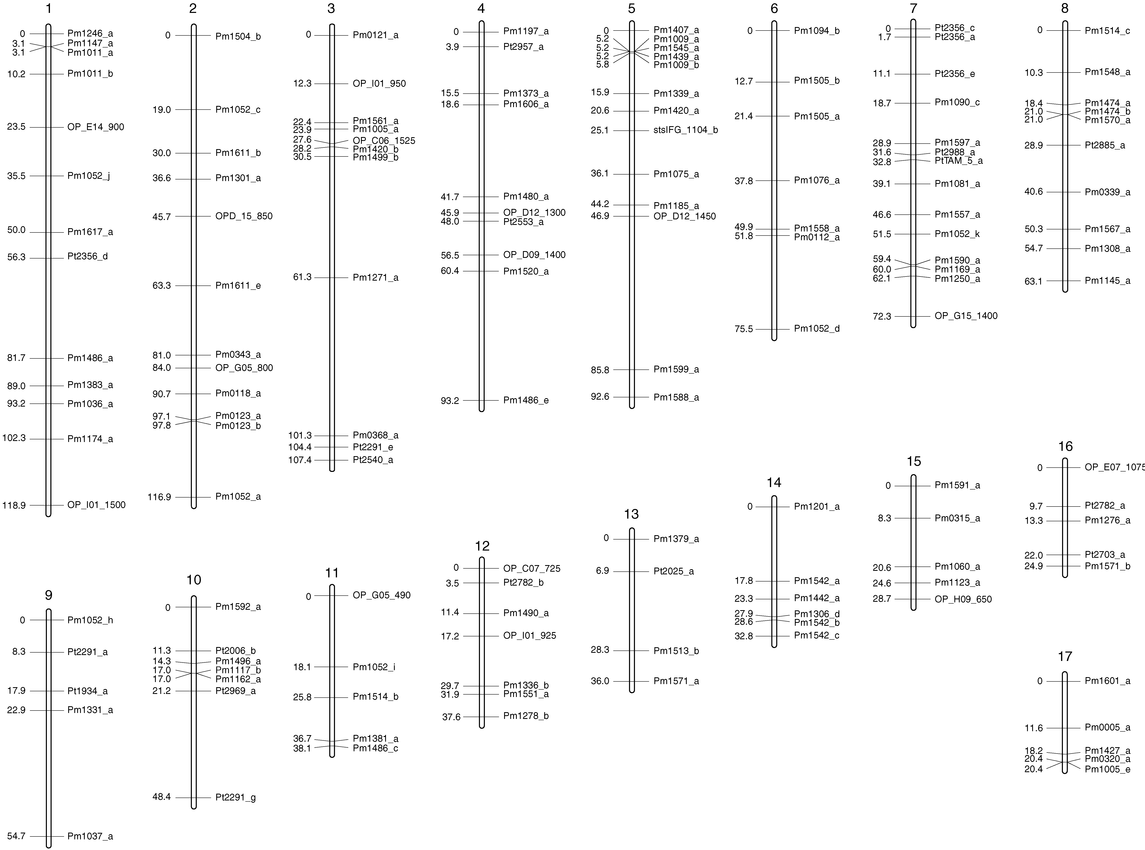
\includegraphics[keepaspectratio, width  =0.8\textwidth]{img/DougFirMap} 
				
\blfootnote{Though we now use molecular markers rather than traits}
\end{frame}





\begin{frame}
			
			\Huge
			Questions? \\ \pause
			Let's take a short break
			
\end{frame}
		
\begin{frame}
\frametitle{Chromosomes}
	\Large \centering	Chromsosomes are the ``particles of inheritence", but what are they made of?
			
		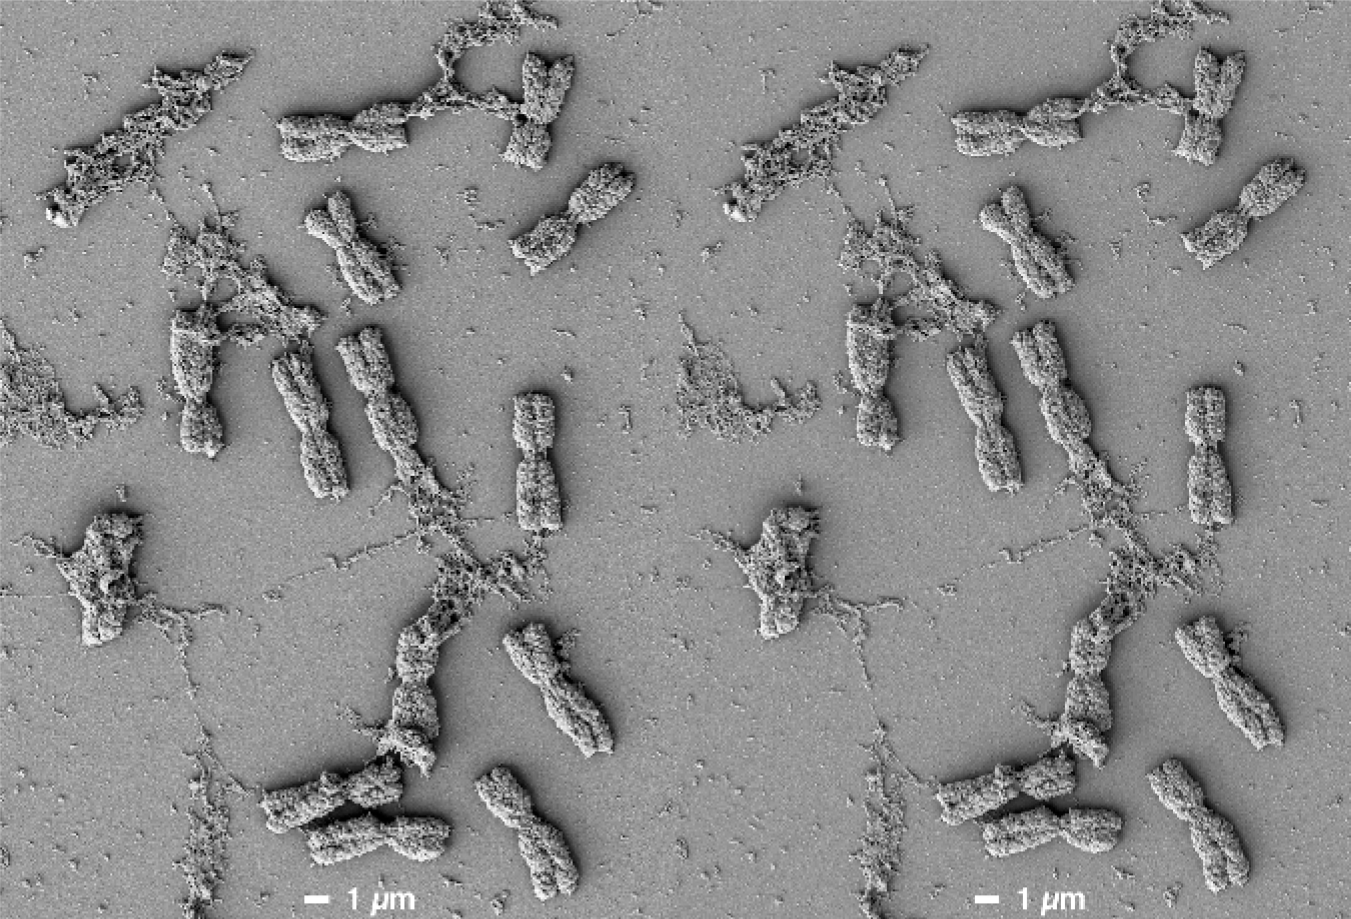
\includegraphics[keepaspectratio, width  =0.8\textwidth]{img/barleyChroms}\blfootnote{SEM of barley chromosomes in metaphase: Schroeder-Reiter and Wanne 2013 \textit{SEM for the Life Sciences}}
	\note{https://www.genome.gov/genetics-glossary/Chromatin}
\end{frame}	

		
		
		\begin{frame}
			\frametitle{A Timeline of Some Discoveries}
			
			\begin{columns}
				\begin{column}{0.4\textwidth}
					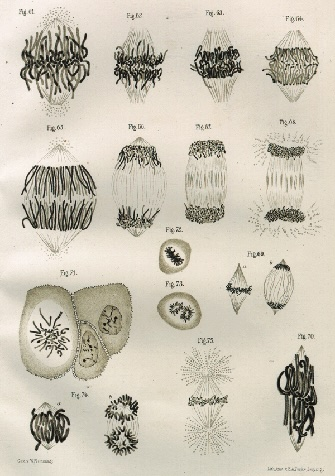
\includegraphics[keepaspectratio, width  =\textwidth]{img/chromosomes}
				\end{column}
				\begin{column}{0.6\textwidth}
					\begin{itemize}
						\small
						\item[1865]  Mendel postulates laws of inheritance 
						\item[1869]  DNA Isolated - though it was unclear what its relevence was unclear 
						\item[1882] Discovery of the fibrous network of "chromatin" (\textit{stainable material}) and chromosomes within nuclei 
						\item[1902-6]  Sutton-Boveri chromosome theory - the segregation of chromosomes during meiosis matches the segregation pattern of Mendel’s laws 
						\item[1915] Morgan demonstrated that chromosomes carry genes, and also discovered genetic linkage\textsuperscript{\textit{won Nobel Prize in 1933}}
						
					\end{itemize}
				\end{column}
				
			\end{columns}
			\blfootnote{Drawing of mitosis by Walther Flemming 1882}
			
			
		\end{frame}
		
		
		
		
		\begin{frame}
			\frametitle{A Timeline of Some Discoveries}
			
			\begin{columns}
				\begin{column}{0.4\textwidth}
					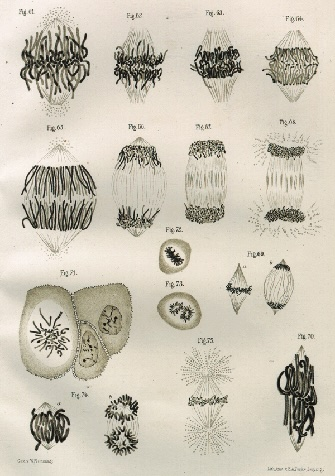
\includegraphics[keepaspectratio, width  =\textwidth]{img/chromosomes}
				\end{column}
				\begin{column}{0.6\textwidth}
					\begin{itemize}
						\small
						\item[1915] Morgan and Sturtevant constructed their genetic map for \textit{D. melanogaster}
						\item[1932] Barbara McClintock confirms that genes are exchanged during crossing-over
						\item[1940s] DNA is determined to be the material within chromosomes that carry heritable information
						\item[1950] The composition of DNA is determined - including Chargaff's rulesf
						
	
						
					\end{itemize}
				\end{column}
				
			\end{columns}
			\blfootnote{Drawing of mitosis by Walther Flemming 1882}
			
			
		\end{frame}
		
		
		
		
		
		\begin{frame}
				\frametitle{Photo 51}
				\centering
			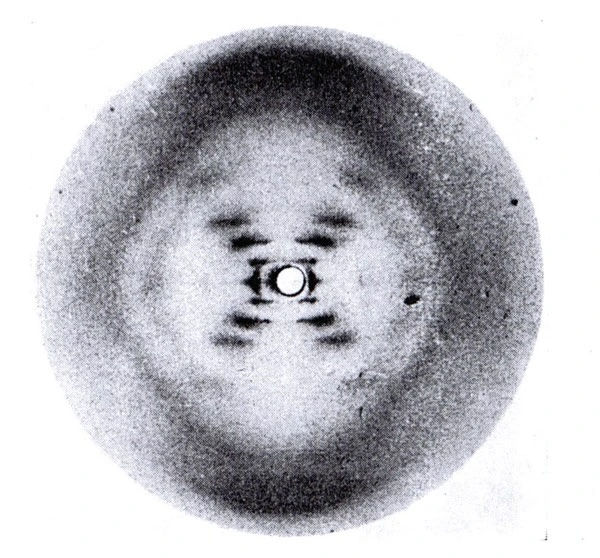
\includegraphics[keepaspectratio, width  =0.75\textwidth]{img/photo_51} 
		\end{frame}
		
		
		\begin{frame}
			\frametitle{Photo 51}
			\centering
			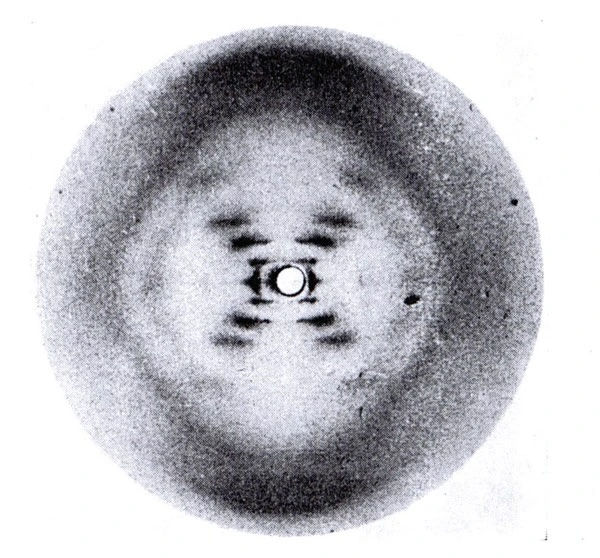
\includegraphics[keepaspectratio, width  =0.75\textwidth]{img/photo_51}  \blfootnote{This photograph, captured by Rosalind Franklin, led directly to the discovery of the structure of DNA}
			
		\end{frame}
	
	
	
	\begin{frame}
		\frametitle{1952-1953 - The Structure of DNA is Determined}
		\begin{columns}
			\begin{column}{0.44\textwidth}
				
				
\begin{itemize}

\small
	\item[--] A molecule of DNA has two strands that form a double helix shape structure, like a twisted ladder
		\item[--] Each step on the ``ladder" is made up of a pair of nitrogenous bases, that are designated with the letters:
		\item[] A – adenine
		\item[] C – cytosine
		\item[] G – guanine
		\item[] T - thimine
	
		
	\end{itemize}		
\end{column}
\begin{column}{0.8\textwidth}
\centering 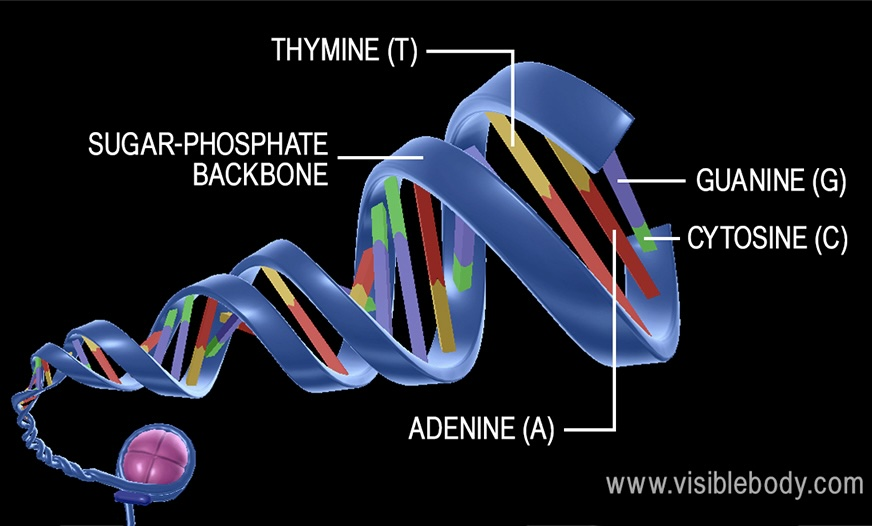
\includegraphics[keepaspectratio, width  =0.75\textwidth]{img/DNA_cartoon}  

\end{column}
\end{columns}
\end{frame}
	
	
	\begin{frame}
			\frametitle{DNA Structure}
\centering 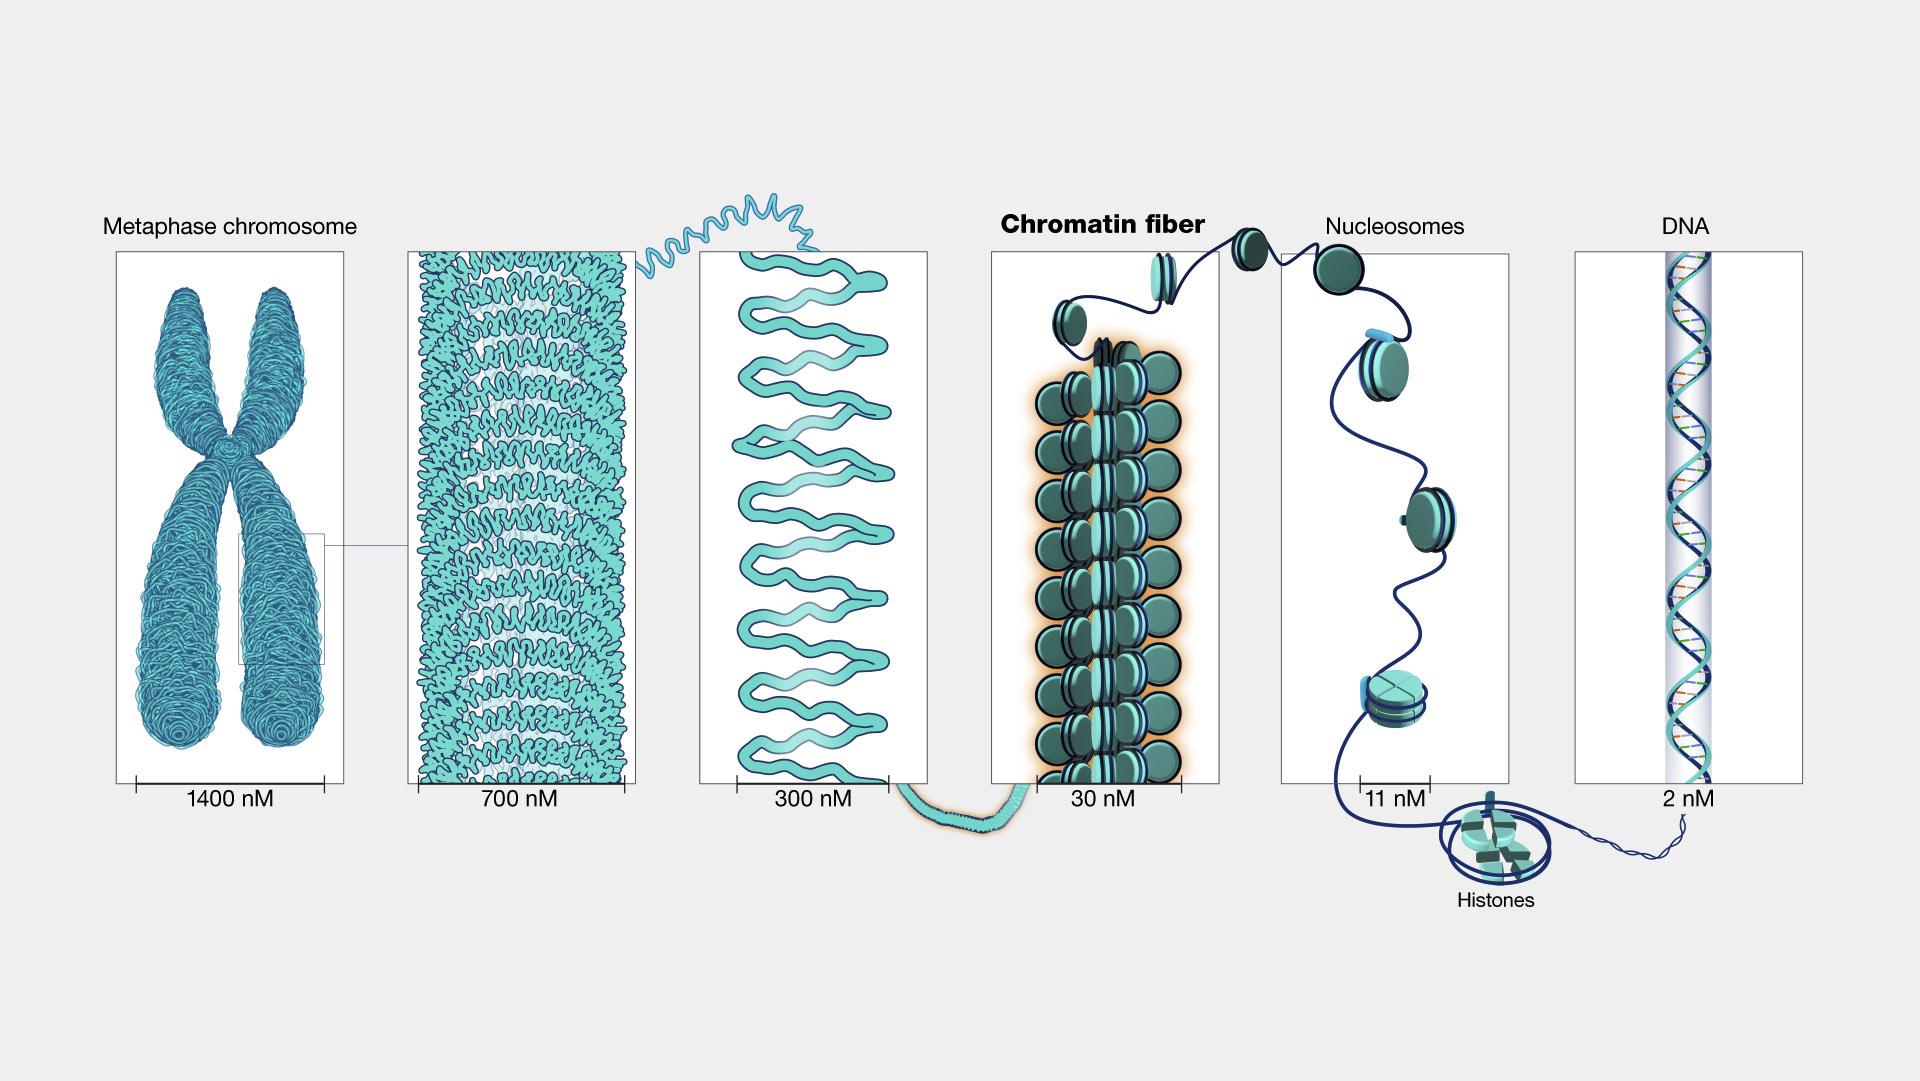
\includegraphics[keepaspectratio, width = \textwidth]{img/chromosomeToDNA}\\


	\end{frame}
	
	
	
	
	\begin{frame}
		
		\frametitle{Question for Next Time}

		Here's a comparison of a genetic map in yeast \textit{Saccharomyces cerevisiae} with an estimate of the physical map (where the genes sit on the DNA itself)\\
		
		\centering	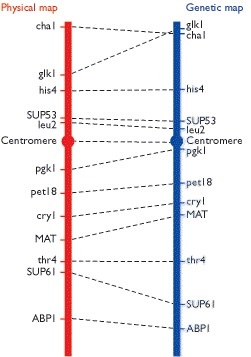
\includegraphics[keepaspectratio, width  =0.37\textwidth]{img/physical_v_genetic} \\
		
		
\textit{		Why would the distances on the genetic map and the physical map differ?}

\blfootnote{Brown 2002, Genomes}
	\end{frame}
	
	
	%%% Slide 17
\end{document}




